\section{Ejercicio Nº 1}

\subsection{Importacion}
\begin{figure}[H]
	\centering
	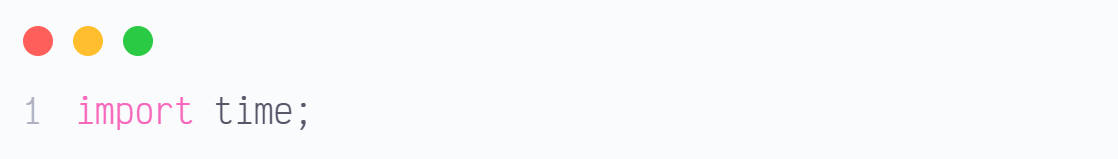
\includegraphics[width=1\textwidth]{Images/code1.png}
	\caption{Importacion de paquete {\color{azulfor} time}.}\label{fig:fg1}
\end{figure}
%====================================================================================================
\subsection{Definiendo Funciones}
\subsubsection{Funcion Lineal}
Nuestra función lineal, calculara la suma de $n$ priemros números consecutivos
mediante la estructura condicional for, iterando $n+1$ veces, realizando una
suma acumulativa.
\begin{figure}[H]
	\centering
	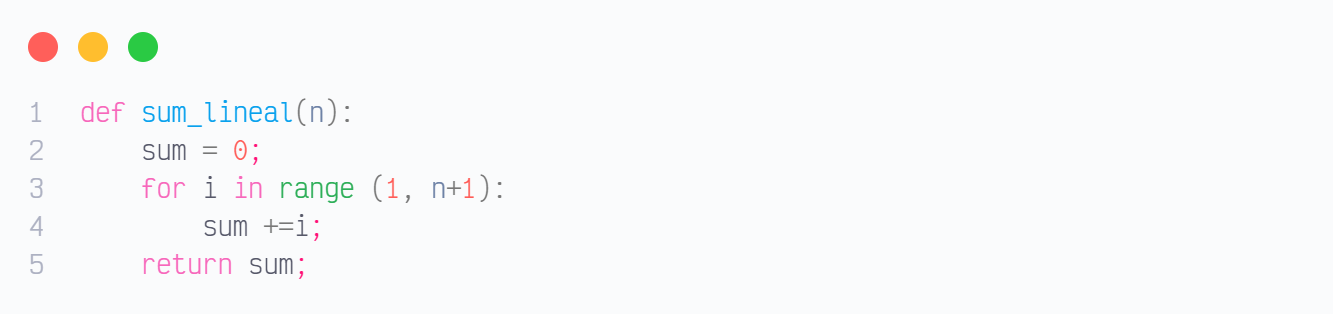
\includegraphics[width=1\textwidth]{Images/code2.png}
	\caption{Definición de la función {\color{azulfor} sum\_lineal}.}\label{fig:fg2}
\end{figure}
%----------------------------------------------------------------------------------------------------
\subsubsection{Funcion Constante}
La función constante realizara la suma de los primeros número enteros
consecutivos mediante la fórmula siguiente:
\[1+2+3+\cdots+n=\cfrac{n(n+1)}{2}\]
\begin{figure}[H]
	\centering
	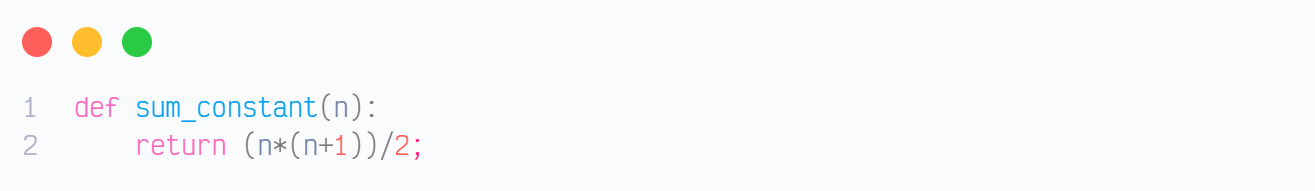
\includegraphics[width=1\textwidth]{Images/code3.png}
	\caption{Definición de la función {\color{azulfor} sum\_constante}.}\label{fig:fg3}
\end{figure}
%====================================================================================================
\subsection{Inicializando y Asignando Valores}
Usaremos 5 eventos para poder experimentar el tiempo de ejecución y así poder
determinar comprobar cual de los algoritmos es más eficiente, óptimo. Los
eventos serán $1000000$, $10000000$, $100000000$, $1000000000$ y $10000000000$,
almacenaremos estos valores en una arreglo de 5 elementos (ver \textbf{Fig
}\ref{fig:fg4}).
\begin{figure}[H]
	\centering
	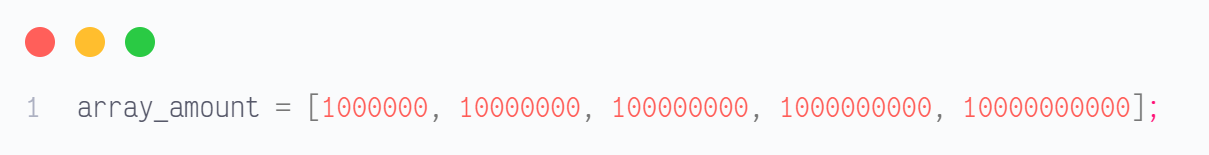
\includegraphics[width=1\textwidth]{Images/code4.png}
	\caption{Para el evento 1}\label{fig:fg4}
\end{figure}
%====================================================================================================
\subsection{Programa Principal}
Esta parte de nuestro código ejecutará las funciones definidas anteriormente
definidas para los cinco eventos. Vamos a recorrer nuestro arreglo elemento por
elemento de la manera mas sencilla podriamos usar un método para recorrer todo
nuestro arreglo y simplificar aún más el código.
\begin{figure}[H]
	\centering
	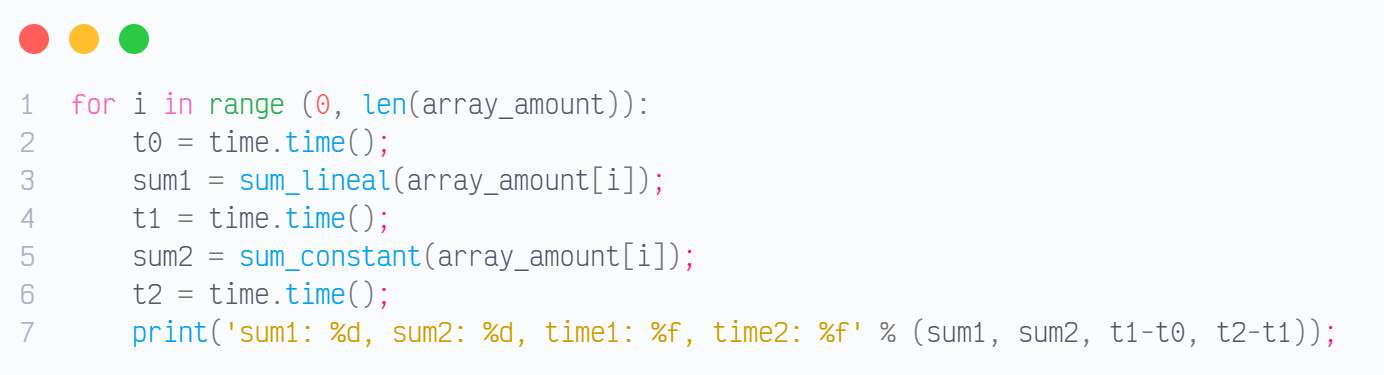
\includegraphics[width=1\textwidth]{Images/code9.png}
	\caption{Programa principal.}\label{fig:fg9}
\end{figure}
%====================================================================================================
\subsection{Ejecución}
Ejecutando nuestro código, hay que tener paciencia para obtener los resultados.

\begin{minipage}{16.2cm}
	\begin{minted}[frame=single,rulecolor=gray,style=perldoc,breaklines,fontsize=\small]{text}
  sum1: 500000500000, sum2: 500000500000, time1: 0.055003, time2: 0.000000
  sum1: 50000005000000, sum2: 50000005000000, time1: 0.611047, time2: 0.000000
  sum1: 5000000050000000, sum2: 5000000050000000, time1: 5.868471, time2: 0.000999
  sum1: 500000000500000000, sum2: 500000000500000000, time1: 63.863117, time2: 0.000000
  sum1: 50000000005000000000, sum2: 50000000005000003584, time1: 1929.456874, time2: 0.000000
	\end{minted}
\end{minipage}

%====================================================================================================
\subsection{Tabla de Resultados}
\begin{table}[H]
	\centering
	\begin{tabular}{L{1.2cm}C{4cm}C{4.5cm}}
		\rowcolor{gray!10}Evento & Tiempo Función Lineal & Tiempo Función Constante \\
		1                        & $0.055003$            & $0.000000$               \\
		2                        & $0.611047$            & $0.000000$               \\
		3                        & $5.868471$            & $0.000999$               \\
		4                        & $63.863117$           & $0.000000$               \\
		5                        & $1929.456874$         & $0.000000$               \\
	\end{tabular}
\end{table}
\cleardoublepage%
%====================================================================================================
\subsection{Conclusiones}
\begin{enumerate}[label=\itemcirccz{azzul}{\arabic*},itemsep=2pt]
	\item La \textbf{\color{azulicg}función constante} (\textbf{Fig.}\ref{fig:fg3}) es
	      más eficiente, óptimo que la \textbf{\color{azulicg}función lineal}
	      (\textbf{Fig.}\ref{fig:fg2}).
	\item En el primer evento la diferencia no se llega a apreciar, a medida que el
	      número aumenta la diferencia se llega a notar, teniendo diferencias muy
	      grandes.
	\item Es recomendable optimizar nuestros algoritmos para en un futruro no tengamos
	      fallos, colapsos, etc. Seria un gran problema.
\end{enumerate}
%====================================================================================================
\subsection{Comentario}
Al momento de tomar la foto del ejemplo no logré capturar el codigo, pero
intenté hacer uno similar, tomando referencia lo aprendido en el curso de
Algoritmos, que llevé con el Ing. Manuel Lagos, en la parte final del curso
realizamos un tema similar.